\section{Conclusion and Discussion}
\subsection{Natural angular frequency}
\subsubsection{Discussions}
    Although we know that the amplitude does not affect the oscillation period, we still try to control the initial position to be the same. It's because little frictional force is unavoidable, which will make the period longer than it should be. As the amplitude gets larger, the negative work done by the frictional force gets more obvious. The third measurement of ten periods is obviously larger tha nthe other three, which might result from the larger amplitude(see Table \ref{data_omega}). However, the experimental value of $\omega_0$ is reliable since its relative uncertainty of is 0.10\%.

\subsubsection{Improvements and recommendations}
    As a device with high precision, the measurement result is quite precise although we only have four measuremnts. Despite that, I suppose controlling the amplitude is necessary to avoid the tiny friction.

\subsection{Damping coefficient}
\subsubsection{Discussions}
    The damping coefficient is calculated from the exponentially decreasing amplitude. In the calculation of damping coefficient, we apply successive difference method to eliminate the deviation. However, the precision is not satisefying because the relative uncertainty reaches 4\%. To be more specific, we want some other data processing methods.

\subsubsection{Improvements and recommendations}
    Besides successive difference method, we can also apply curve fitting in this case. By exponential cauve fitting, we can also obtain the damping coefficient $\beta$ from $\theta_n=\theta_0e^{-\beta (nT)}$.
    \begin{figure}[H]
    \centering
        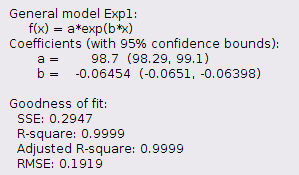
\includegraphics[width=0.55\textwidth]{images/fitting}
        \caption{Fitting curve information for $\beta$}\label{fitting}
    \end{figure}
    From the information of the exponential fitting cure, we find that its R-square value is quite close to 1, which means it's very likely to be an exponential function. We notice that the b value here, which presents $-\beta$, is $-0.06454\pm 0.0006s^{-1}$. Compared with our result by successive difference method $\beta=0.0657\pm 0.003s^{-1}$, the fitting value is more preicise. It shows that different methods to obtain some values are different in precision and reliability.

\subsection{$\varphi$ vs. $\omega$}
\subsubsection{Discussions}
    Both of the $\varphi$ vs. $\omega$ curve are decreasing in the shape of arc cotangent (see Figure \ref{phi}). In theory we know that for the smaller damping coefficient, the left side curve of $\omega/\omega_0=1.0$ is higher than the other and the right side curve is lower than that. However, our results show that although the right half of the damping selection 3 curve is higher than damping selection 2 near the $\omega/\omega_0=1.0$, its gets lower quickly and beneath the damping selection 2, which is abnoraml. We recall the measurement procedure and conclude that it's blamed on the backslash error. During the second half of the experiment we thought the $\omega$ gap we chose is too small so we relatively quickly rotated the knob but made the gap too big. Therefore, we rotated the knob inversely to measure the middle $\omega$ again. Also, the time duration will be longer to reach the stable situation. This causes the second half of phase shifts to be smaller.

\subsubsection{Improvements and recommendations}
    During the experiment we find it hard to predict the phase shift. We can only see the strobe flashes and read the phase shift. There are two methods to this problem.
    \begin{enumerate}
        \item Rotate the knob very carefully and be patient enough to read the phase shift for more times until it's stable. Patience can eliminate the deviation.
        \item Redesign the machine. If there's an easier way to directly change the phase shift to the expected value, the entire experiment will be easy.
    \end{enumerate}
    Whichever improvement we make, we have to be patient to ensure the oscillation is stable.

\subsection{$\theta_{st}$ vs. $\omega$}
\subsubsection{Discussions}
    The shape of both curve are within our expectation (see Figure \ref{theta}). Obviously, the damping coeffiecient 2 is smaller than damping coeffiecient 3 beacuse the entire curve of damping selection 2 is above the curve of damping selection 3. we find that their beginning are roughly the same. However, it's hard to tell whether the peaks occur on the left or right hand side of the straight line $\omega/\omega_0=1.0$. In our expectation, the peaks should occur on the slightly left of the straight line. We suppose it's because the oscillation has not been stable yet. The value of $10T$ is smaller so that the calculated $\omega$ is larger than the real value, which makes the entire curve move rightwards. Therefore, the peak does not occur on the slightly left of $\omega/\omega_0=1.0$.

\subsubsection{Improvements and recommendations}
    Sometimes we found the amplitude changes right after we recorded the periods. In order to make the result accurate, we still need patience. 